\subsection{Geração de Malhas}

Para que seja possível aplicar o método dos elementos finitos, é necessário discretizar o domínio em elementos. O domínio discretizado  chama-se malha, sobre a qual as simulações numéricas de escoamento devem ser executadas. A Fig. \ref{fig:perfuracao} ilustra a perfuração de um poço de petróleo, onde a região com hachuras em amarelo caracteriza o domínio a ser modelado.
\begin{figure}[H]
	\centering
	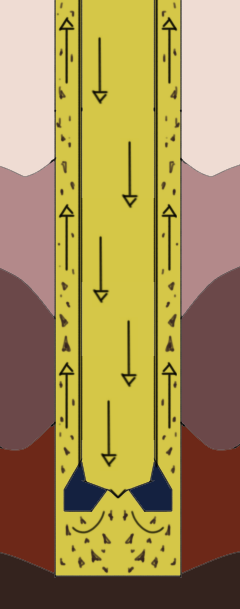
\includegraphics[scale=0.6]{img/broca.png}
	\caption[Ilustração de uma perfuração de um poço de petróleo.]{Ilustração de uma perfuração de um poço de petróleo. Fonte: autor}
	\label{fig:perfuracao}
\end{figure}


A Fig. \ref{fig:desenho_referencia_broca} é uma representação esquemática de um poço de petróleo, cuja ilustração foi utilizada como referência para criar o domínio geométrico no software AutoCad e, a partir dele, gerar o malhamento triangular. As setas representam o sentido do escoamento. As dimensões do revestimento são: 8,66 pol (aproximadamente 0,220 m) de largura e 39,37 polegadas (aproximadamente 1 m) de comprimento \cite{Rocha}. Simplificadamente, o comprimento do revestimento foi limitado a 1 m de extensão e a rugosidade na parede da formação simulada como uma interpolação por \textit{spline} de pontos definidos ``quase-aleatórios''.
\begin{figure}[H]
	\centering
	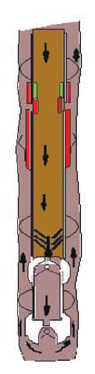
\includegraphics[scale=0.7]{img/casing1.png}
	\caption[Representação esquemática de um poço de petróleo.]{Representação esquemática de um poço de petróleo \cite{Erik}.}
	\label{fig:desenho_referencia_broca}
\end{figure}

A Fig. \ref{fig:contornos} é o resultado do desenho no AutoCad do modelo simétrico com $\varsigma$ máximo, posteriormente editada no software Paint para evidenciar o sentido do escoamento dos fluidos, bem como os contornos de entrada (\textit{inflow}) e saída (\textit{outflow}) de fluido – em verde e azul –, e também as paredes (\textit{wall}) – em marrom.
\begin{figure}[H]
	\centering
	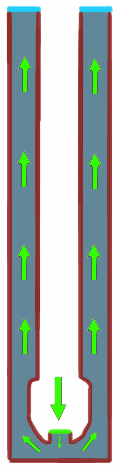
\includegraphics[scale=0.7]{img/broca_petroleo_formacao_lisa_autocad2.png}
	\caption[Representação dos contornos da malha.]{Representação dos contornos da malha. Fonte: autor.}
	\label{fig:contornos}
\end{figure}

Utilizamos o software Gmsh para gerar a malha \cite{Gmsh}. Gmsh é um programa de código aberto com o objetivo de gerar malha de elementos finitos 1D, 2D e 3D com suporte integrado a CAD. A filosofia por detrás do Gmsh é contribuir com a facilidade e rapidez na construção de uma malha. Para criar modelos, pode-se usar a interface gráfica ou a sua própria linguagem nativa por meio de \textit{scripts}. Há também uma API para as linguagens de programação C/C++, Python e Julia \cite{Gmsh}. Apesar disso, a facilidade de se trabalhar e a quantidade de recursos superior do AutoCad motivaram-nos escolhê-lo para construir o modelo. O modelo geométrico é dividido em vários elementos, tais como pontos, linhas, triângulos, quadriláteros, tetraedros e hexaedros, conectados entre si por vértices, ou nós. O Gmsh implementa vários algoritmos para gerar malhas automaticamente. As malhas em geral são não estruturadas. isto é, não existe nenhuma relação predefinida entre quaisquer dois elementos \cite{GmshDocuments}.

O Gmsh pode ler muitos tipos de arquivos. Um deles é o formato IGES, exportável pelo AutoCad. Portanto, para que haja integração entre o Gmsh e o AutoCad, trabalhamos com arquivos do tipo IGES. Normalmente, é útil combinar alguns elementos geométricos em grupos com o objetivo de definir propriedades matemáticas, tais como domínio, condições de contorno, funcionais ou materiais. Esse agrupamento pode ser feito no módulo \textit{Geometry} do Gmsh através do estabelecimento de "grupos físicos".

Para as malhas consideradas aqui, definimos 4 grupos físicos: \texttt{inflow}, \texttt{outflow}, \texttt{wall} e \texttt{flow}. Como já dissemos, o primeiro e o segundo grupo correspondem à entrada e saída de fluido. As paredes do poço, a saber, a formação rochosa nua, bem como as paredes do revestimento são tratadas pela condição de não escorregamento (\textit{no-slip}), onde a velocidade é assumida nula. Por fim, o interior do domínio, \texttt{flow}, é tratado como uma superfície física. Todas as malhas são não estruturadas e compostas de elementos triangulare com refinamento adaptativo na região de \texttt{inflow} próxima à sapata, conforme mostra a Fig. \ref{fig:malha_A_B}. Como fase final, exportamas as malhas no formato \texttt{.msh} para, em seguida, serem processadas no \textit{solver} da biblioteca FEniCS. 

%As simulações numéricas foram realizadas para diferentes tipos de geometria de poços, casos em que a formação é lisa e casos em que há um certo grau de rugosidade. Também são simulados casos de Standoff menor que 100\%, isto é, o revestimento não está perfeitamente centralizado, como foi explicado no capítulo sobre Standoff. Após as simulações numéricas, são comparados a eficiência do colchão lavador, nas diferentes geometrias de poço, por um parâmetro de eficiência de limpeza.

Consideramos 4 modelos, aqui denominados $A_1$, $A_2$, $B_1$ e $B_2$, cujas dimensões são iguais, com 1 metro de altura e 0.22 metros de comprimento, as condições iniciais e de contorno são idênticas. As propriedades do fluido simulado também são as mesmas para todas as geometrias, assim como os parâmetros de simulação. Os modelos $A$ possuem paredes lisas, ao passo que os modelos $B$ admitem rugosidades. Para os modelos $A_1$ e $B_1$, $\varsigma = 100\%$; 
para $A_2$ e $B_2$, $\varsigma < 100\%$. As malhas $A$ são representadas na figura Figs. \ref{fig:malha_A_B} com expansão da região da base do poço. As malhas $B$ são representadas na Fig.
\ref{fig:malha_C_D} também com expansão da região da base do poço, ilustrando as diferentes malhas utilizadas.
\begin{figure}[H]
	\centering
	\begin{subfigure}[b]{0.1\linewidth}
		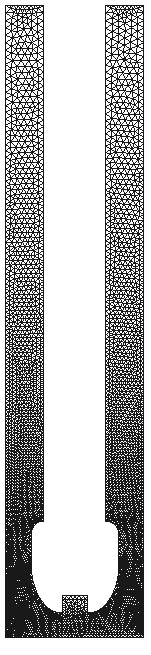
\includegraphics[width=\linewidth]{img/lisa.png}
	\end{subfigure}	
	\quad
	\quad
	\quad
	\quad
	\quad
	\begin{subfigure}[b]{0.1\linewidth}
		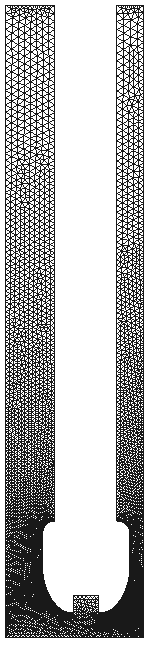
\includegraphics[width=\linewidth]{img/lisa_standoff.png}
	\end{subfigure}
	\\
	\begin{subfigure}[b]{0.3\linewidth}
		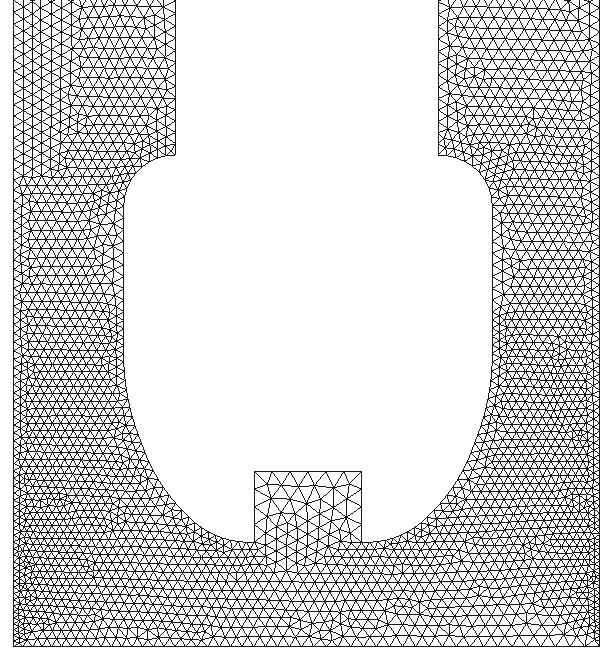
\includegraphics[width=\linewidth]{img/lisa_sapata.png}
	\end{subfigure}
	\quad
	\quad
	\quad
	\quad
	\quad
	\begin{subfigure}[b]{0.3\linewidth}
		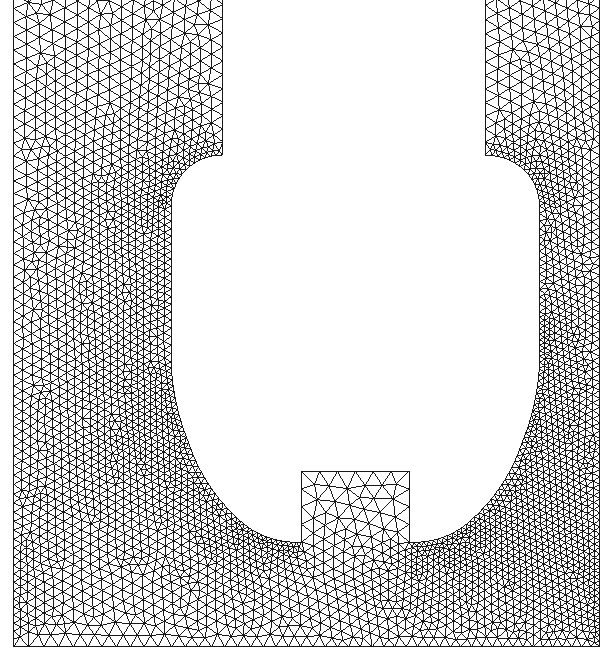
\includegraphics[width=\linewidth]{img/lisa_standoff_sapata.png}
	\end{subfigure}

	\caption[Malhas da configuração $A$: anular e sapata.]{Malhas da configuração $A$: anular e sapata. Fonte: autor.}
	\label{fig:malha_A_B}
\end{figure}

\begin{figure}[H]
	\centering
	\begin{subfigure}[b]{0.1\linewidth}
		\includegraphics[width=\linewidth]{img/rugosa.png}
	\end{subfigure}
	\quad
	\quad
	\quad
	\quad
	\quad
	\begin{subfigure}[b]{0.1\linewidth}
		\includegraphics[width=\linewidth]{img/rugosa_standoff.png}
	\end{subfigure}
	\\
	\begin{subfigure}[b]{0.3\linewidth}
		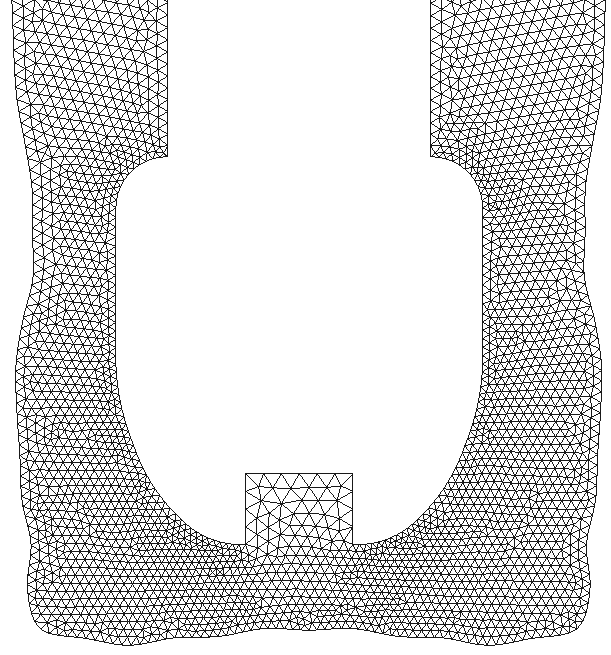
\includegraphics[width=\linewidth]{img/Rugosa_sapata.png}
	\end{subfigure}
	\quad
	\quad
	\quad
	\quad
	\quad
	\begin{subfigure}[b]{0.3\linewidth}
		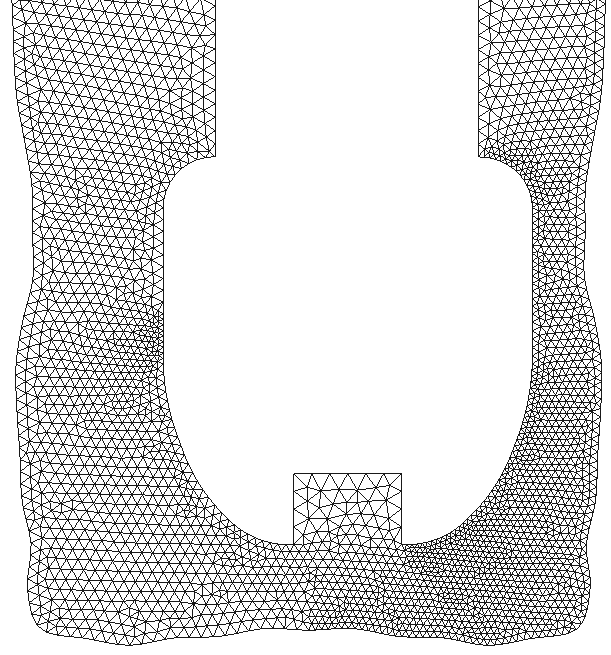
\includegraphics[width=\linewidth]{img/Rugosa_standoff_sapata.png}
	\end{subfigure}
	\caption[Malhas da configuração $B$: anular e sapata.]{Malhas da configuração $B$: anular e sapata. Fonte: autor.}
	\label{fig:malha_C_D}
\end{figure}
\noindent A Tab. \ref{tab:Geo_Valor_Standoff} resume os principais parâmetros de malha e a taxa de \textit{standoff} considerados para cada modelo. Onde $n_{elem}$, $n_{ver}$ e $n_{nos}$ é o número de elementos, de vértice e de nós da malha, respectivamente.
\begin{table}[h!]
    \centering
    \caption{Principais parâmetros de malha.}
    \begin{tabular}{ccccc}
    \hline
    modelo & $n_{elem}$ & $n_{ver}$ & $n_{nos}$ & $\varsigma$ \\
    \hline
    $A_1$ & 12520 & 6698 & 44828 & 100\% \\
    $A_2$ & 12986 & 6931 & 40458 & 50\% \\
    $B_1$ & 14706 & 7810 & 53278 & 100\% \\
    $B_2$ & 14550 & 7732 & 52654 & 50\% \\
    \hline
    \end{tabular}
    \label{tab:Geo_Valor_Standoff}
\end{table}

foi utilizado elementos triangulares de Taylor-Hood \cite{Taylor} com interpolação quadrática para a velocidade e interpolação linear para a pressão. Esses elementos são denotados como P2P1. Além de estáveis, esses elementos também convergem quadraticamente. Cada componente de velocidade será caracterizada por 6 nós enquanto a pressão será caracterizada por 3 nós Fig. \ref{fig:elements}

\begin{figure}[H]
	\centering
	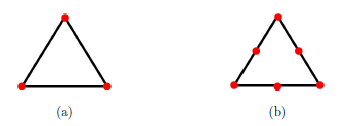
\includegraphics[scale=1]{img/elements.png}
	\caption[Representação dos contornos da malha.]{Elementos de triângulo linear e quadrático. A figura (a) corresponde aos elementos lineares de pressão e a figura (b) corresponde aos elementos quadráticos para cada componente da velocidade. Fonte: \cite{Cornthwaite}}
	\label{fig:elements}
\end{figure}